\documentclass{acmsiggraph}               % final
%\documentclass[review]{acmsiggraph}      % review
%\documentclass[widereview]{acmsiggraph}  % wide-spaced review
%\documentclass[preprint]{acmsiggraph}    % preprint

%% Uncomment one of the four lines above depending on where your paper is
%% in the conference process. ``review'' and ``widereview'' are for review
%% submission, ``preprint'' is for pre-publication, and ``final'' is for
%% the version to be printed.

%% These two line bring in essential packages: ``mathptmx'' for Type 1 
%% typefaces, and ``graphicx'' for inclusion of EPS figures.

\usepackage{mathptmx}
\usepackage{graphicx}

%% use this for zero \parindent and non-zero \parskip, intelligently.

\usepackage{parskip}
\usepackage{subfigure}
\usepackage{smrdefaults}

%% If you are submitting a paper to the annual conference, please replace 
%% the value ``0'' below with your OnlineID. If you are not submitting this
%% paper to the annual conference, you may safely leave it at ``0'' -- it 
%% will not be included in the output.

\onlineid{0}

%% need to document this!

\acmformat{print}

%% Paper title.

\title{TAPESTREA: Sound Scene Modeling By Example}

%% Author and Affiliation (single author).

\author{Ananya Misra, Perry R. Cook, and Ge Wang\\Princeton University\thanks{e-mail: \{amisra, prc, gewang\}@cs.princeton.edu}}

%% Author and Affiliation (multiple authors).

%%\author{Roy G. Biv\thanks{e-mail: roy.g.biv@aol.com}\\ Starbucks Research %
%%\and Ed Grimley\thanks{e-mail:ed.grimley@aol.com}\\ Grimley Widgets, Inc. %
%%\and Martha Stewart\thanks{e-mail:martha.stewart@marthastewart.com}\\ Martha Stewart Enterprises \\ Microsoft Research}

%% Keywords that describe your work.

\keywords{sound texture, synthesis, sinusoidal modeling, wavelet}

%%%%%% START OF THE PAPER %%%%%%

\begin{document}

\teaser{
\center
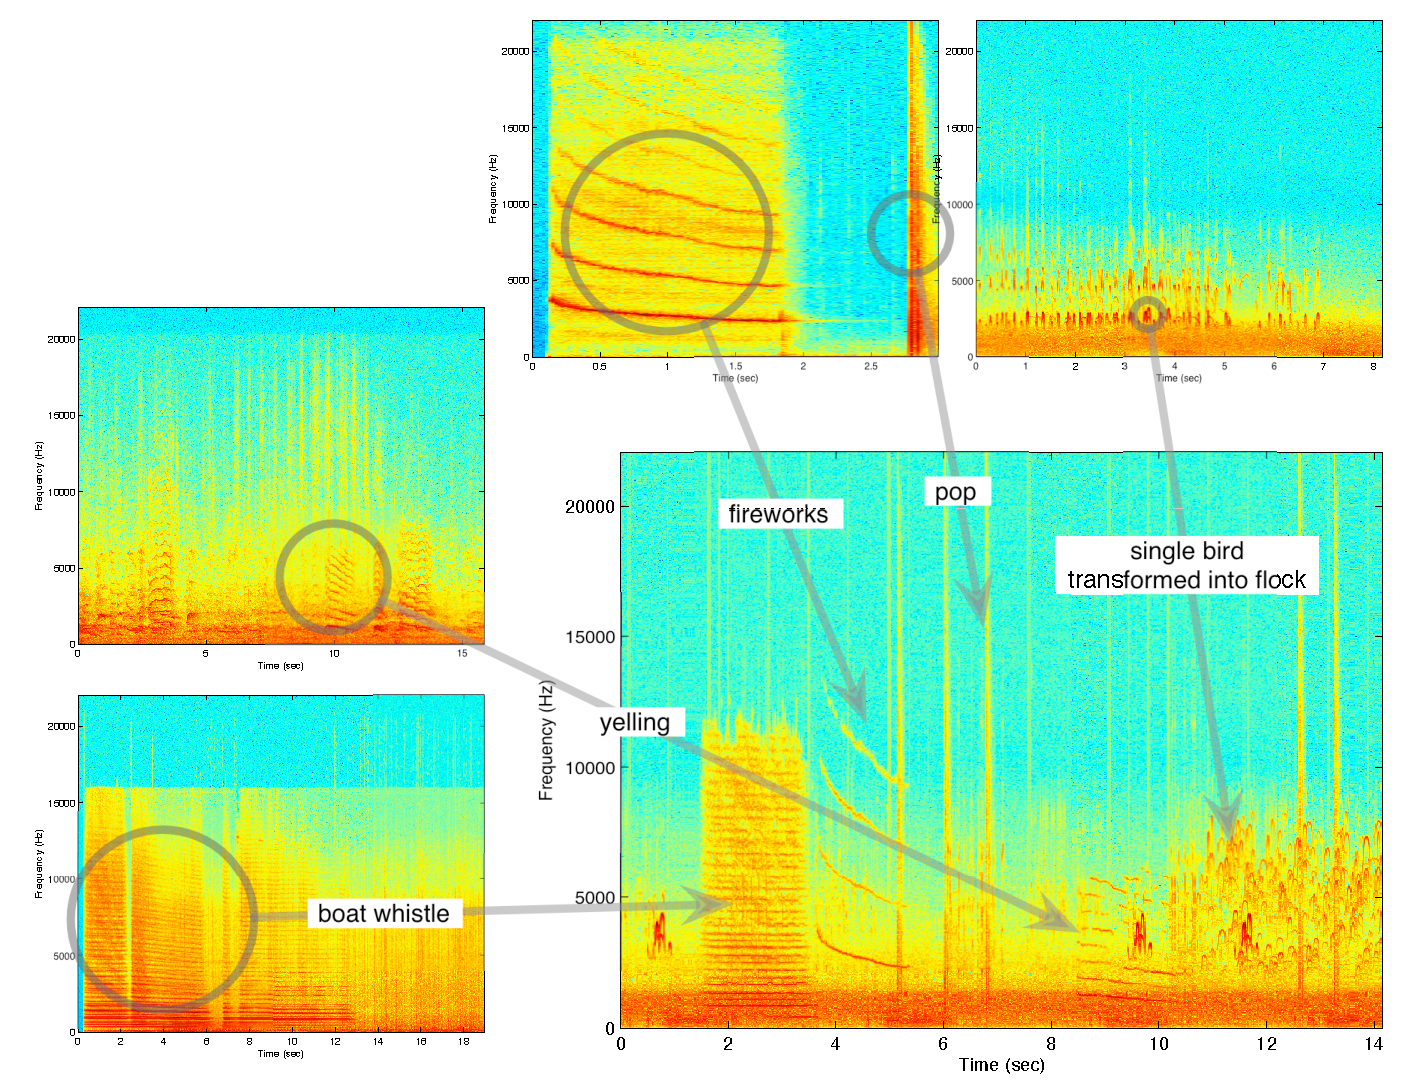
\includegraphics[width=6.5in]{teaser.eps}
%  \subfigure[original]{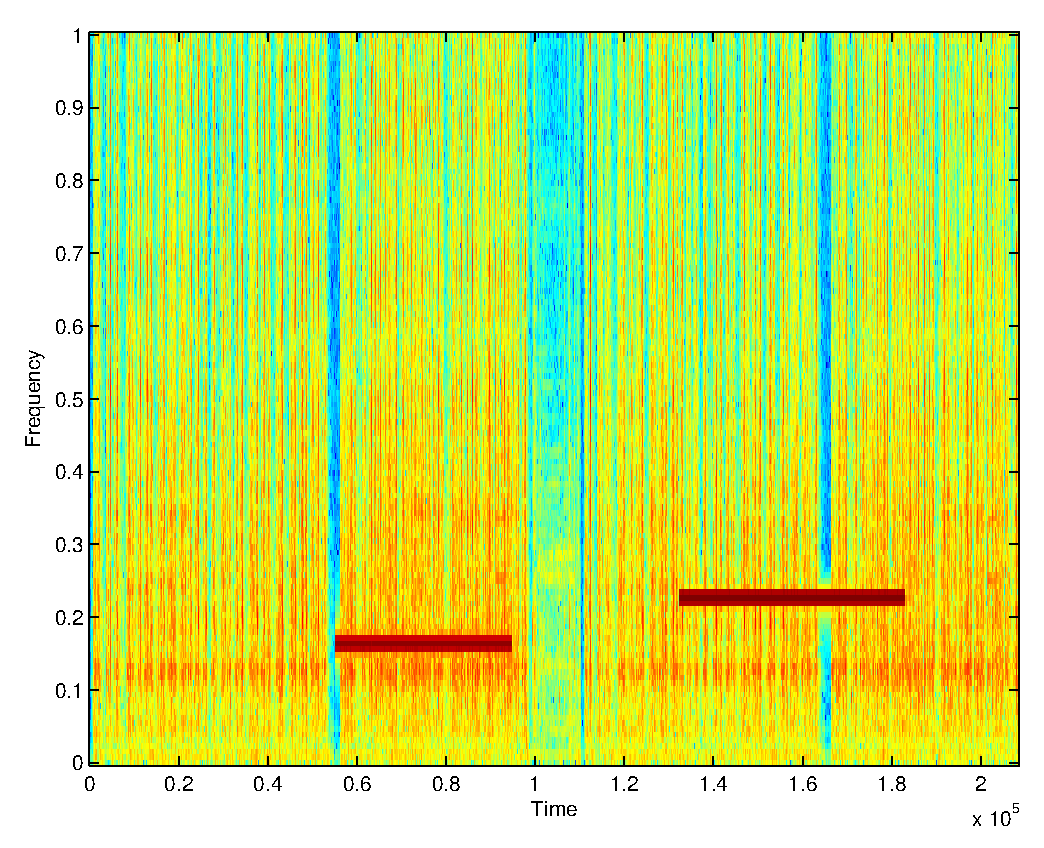
\includegraphics[width=.24\textwidth]{story1.eps}}
%  \subfigure[foreground]{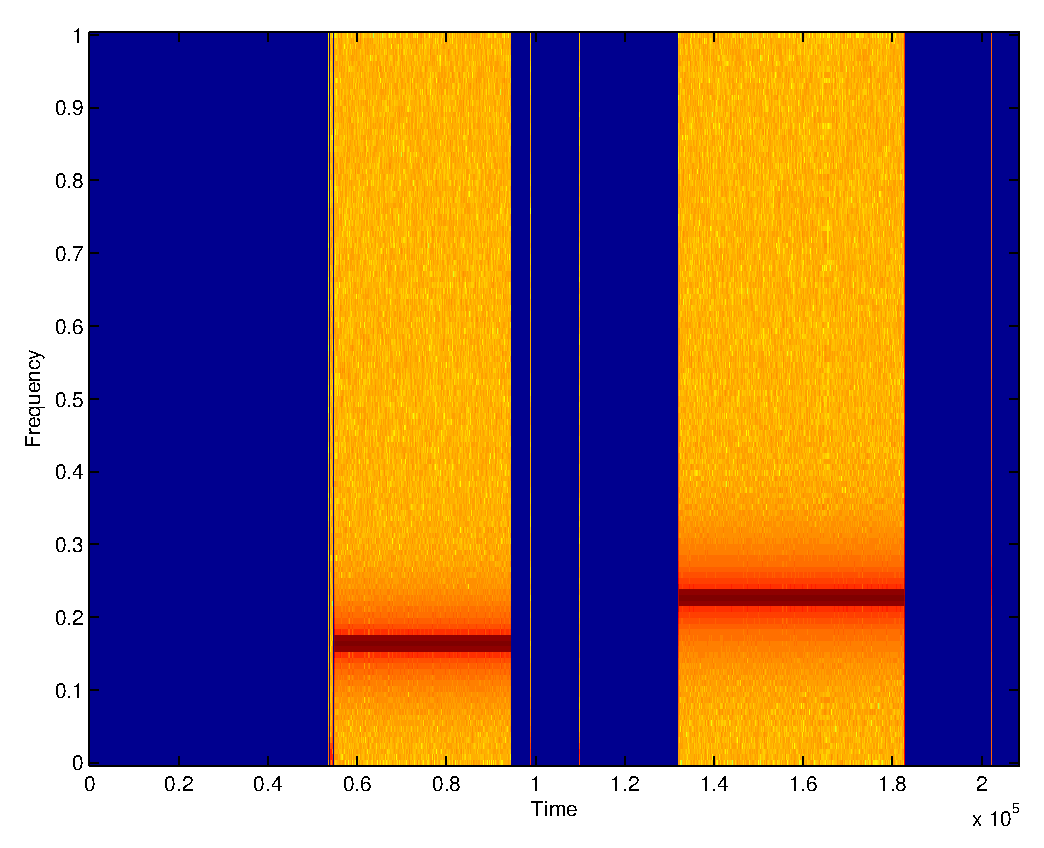
\includegraphics[width=.24\textwidth]{story2.eps}}
%  \subfigure[background]{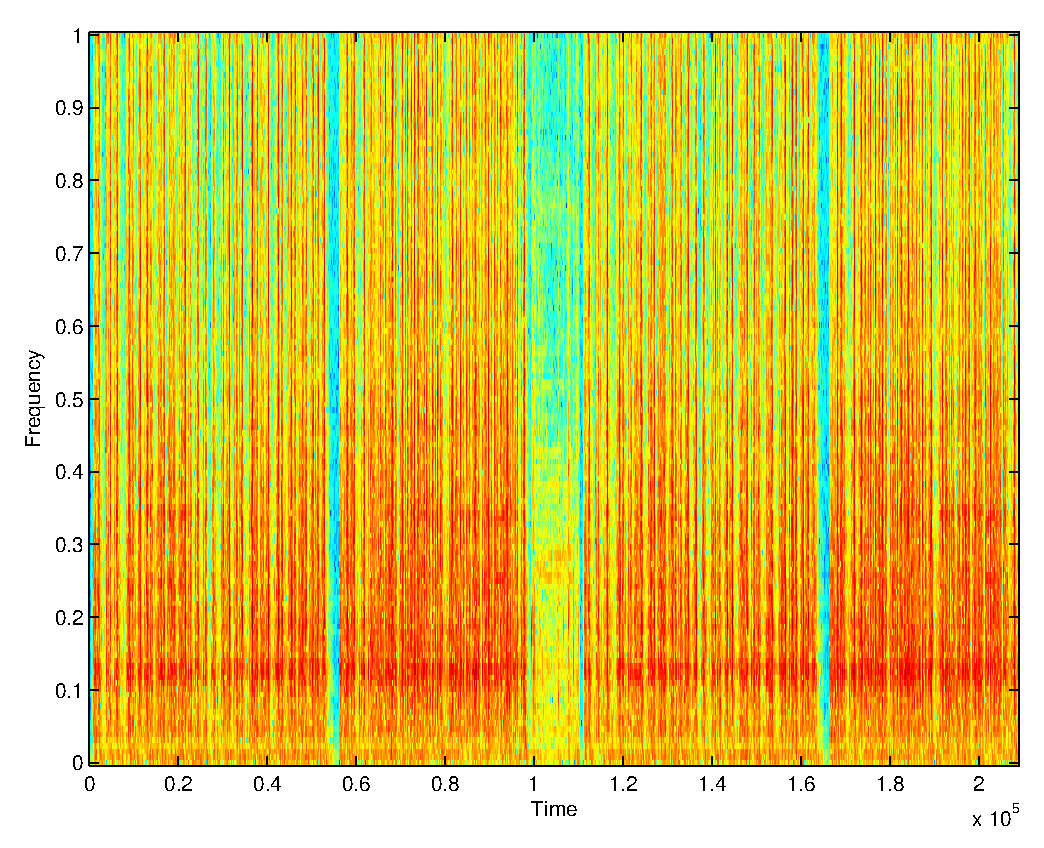
\includegraphics[width=.24\textwidth]{story3_fake.eps}}
%  \subfigure[synthesized]{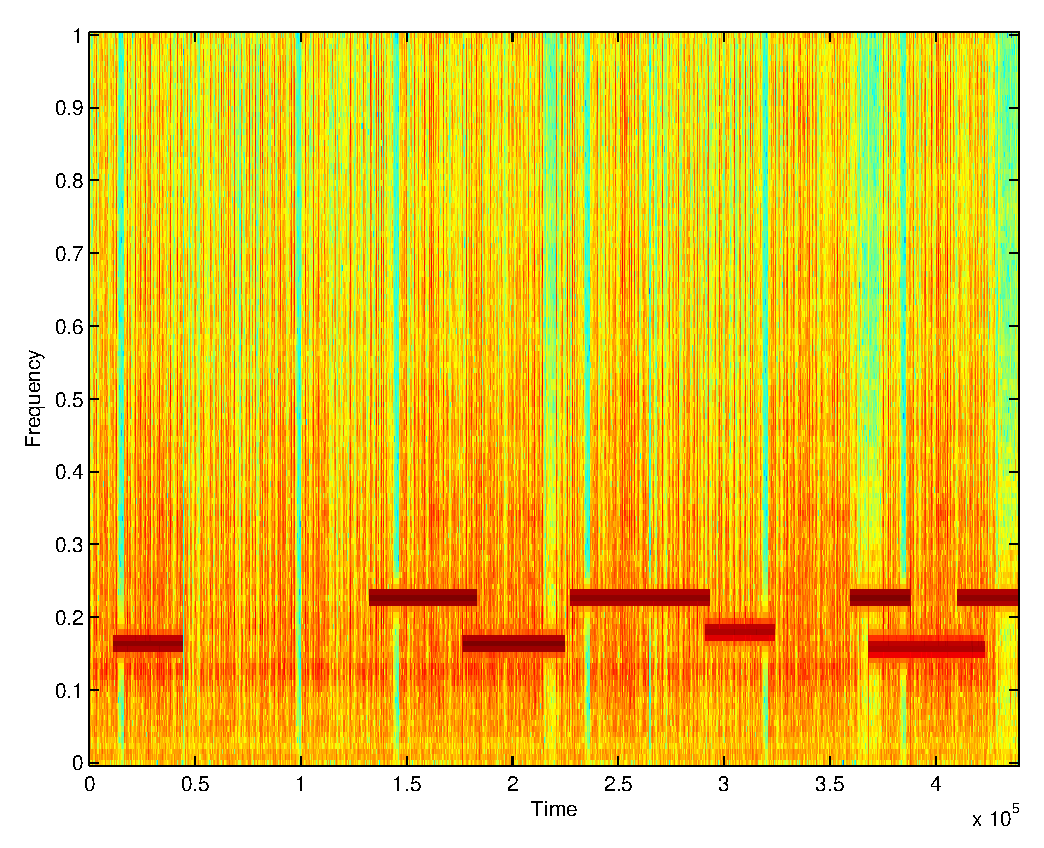
\includegraphics[width=.24\textwidth]{story4_fake.eps}}
 \caption{ hi there. }
}
%\teaser{

% The ``\maketitle'' command must be the first command after the
% ``\begin{document}'' command. It prepares and prints the title block.

\maketitle

% Abstract section.

\begin{abstract}

%This paper is abstract (in many ways).
% data-driven - should we add?

A sound scene can be defined as any "environmental" sound that has a 
consistent background texture, with one or more potentially recurring 
foreground events.  We describe a data-driven framework for analyzing, 
transforming, and synthesizing high-quality sound scenes.  The framework 
provides flexible control over the various components that make up the 
synthesized sound.  Given one or more sound scenes, our system provides 
well-defined means to:  (1) automatically or interactively select points 
of interest in the sound and extract them into reusable templates,  (2) 
transform sound components independently of the background and/or other 
events, (3) continually re-synthesize the background texture in a 
perceptually-convincing manner, and (4) controllably place event 
templates over the background, varying key parameters such as density, 
periodicity, relative loudness and spatial positioning of the 
components.  Our main contributions includes techniques and paradigms 
for (1), (2), and (4), extensions to a wavelet-based algorithm used in 
(3), and an interface to facilitate the various phases in our approach.  
Given this framework, it is possible to completely transform an existing 
sound scene, dynamically generate sound scenes of unlimited length, and 
constructnew sound scenes by combining elements from different existing 
sound scenes.

%We describe a framework for synthesizing perceptually-convincing sound 
%scenes of unlimited length, with fine control over the characteristics 
%and occurrences of individual foreground events and the qualities of the 
%sound scene.  Given one or more example sounds, the system can 
%automatically locate and isolate deterministic (sinusoidal) events, 
%transient events, and background textures into reusable templates.  Our 
%framework also allows users to interactively highlight points of 
%interest in the sound for event isolation, manipulate events 
%independently, change the density of events, and even create new sound 
%scenes by combining elements of different source templates.  

%Our general approach models foreground events and background sound 
%separately. We apply  spectral modeling to extract deterministic  
%sinusoidal events and a stochastic residue from the given sound.  The 
%deterministic events are then generated to order, possibly after 
%spectral transformations, using sinusoidal resynthesis. The 
%stochastic component may also contain non-sinusoidal events, known as 
%\textit{transients}. We generate the stochastic component using wavelet 
%tree learning. The resulting system provides a new paradigm for 
%interactively synthesizing high-quality sound texture with flexible 
%control over the variety and quality of the synthesized sound.

%Citations can be done this way~\cite{Jobs95} or this more concise 
%way~\shortcite{Jobs95}, depending upon the application.
\end{abstract}

% ACM Computing Review (CR) categories. 
% See <http://www.acm.org/class/1998/> for details.
% The ``\CRcat'' command takes four arguments.

%\begin{CRcatlist}
%  \CRcat{K.6.1}{Management of Computing and Information Systems}%
%{Project and People Management}{Life Cycle};
%  \CRcat{K.7.m}{The Computing Profession}{Miscellaneous}{Ethics}
%\end{CRcatlist}

% The ``\keywordlist'' command prints out the keywords.
\keywordlist

\section{Introduction}
% The ``\copyrightspace'' command must be the first command after the 
% start of the first section of the body of your paper. It ensures the
% copyright space is left at the bottom of the first column on the first
% page of your paper.
%\copyrightspace
Many sound synthesis techniques focus on generating foreground sounds 
such as voices, music, or sudden events that attract our attention. 
These sounds alone do not generally give the listener a strong sense of 
being in a real-world environment where there are many background noises as 
well. The totality of sounds that compose an auditory scene is the focus 
of the work described in this paper.  Existing methods that deal with 
pre-recorded sound do not provide the suitable level of 
analysis/synthesis techniques to allow truly flexible "sound scene 
modeling by example," where a sound scene can be composed from selected 
components of different example sounds. This is analogous to the 
data-driven surface construction approach used in 3D geometric modeling 
by example  ~\cite{Funkhouser04}. 

A sound texture can be described as a sound with structural elements 
that repeat over time, but with some randomness. The randomness prevents 
it from being modeled well by strictly deterministic techniques. On the 
other hand, the sound cannot be modeled as a purely random process since 
on some level it appears stationary, but has distinguishing 
characteristics that are not purely random. Textures often form a large 
part of the background of sound scenes.

Sound scene synthesis is the creation of perceptually convincing sounds 
based on a set of example sounds. The generated sound should be 
arbitrarily close to the original, so that it can either be perceived as 
another instance of it, or as a completely different scene. Since 
repeatedly playing the original sound is not convincing, the synthesis 
should involve some randomness as well as a flexible amount of user control. 
%/*The generated sound should be sufficiently like the original to be perceived 
%as another instance of it. However, merely repeatedly playing the original sound is not 
%convincing, so the synthesis should also involve some randomness. */

Given one or more example sound scenes, we would like to generate from 
these an unlimited supply of non-repeating, perceptually convincing 
sound that can be parametrically controlled to fit the user's 
specifications. One of our goals is to provide an automation tool for 
easily modeling and generating sound textures and scenes for 
entertainment (movies, TV, and games), Virtual and Augmented Reality, 
and art projects such as live perfor mances and installations.

Towards this aim, we introduce TAPESTREA: Techniques and Paradigms for 
Expressive Synthesis, Transformation and Rendering of Environmental 
Audio. Our general approach is based on the notion that sound scenes are 
composed of events as well as background sound, which are best modeled 
separately. We apply spectral modeling ~\cite{Serra89} to extract 
deterministic sinusoidal events and a stochastic residue from a given 
sound. The deterministic events are then generated to order, possibly 
after spectral transformations, using sinusoidal resynthesis. The 
stochastic component may also contain brief non-sinusoidal events 
(transient) events.  We optionally isolate and extract transients as 
well. Once deterministic and transient events are separated from the 
background, we generate the stochastic background component using a 
wavelet tree learning algorithm by Dubnov et. al. ~\shortcite{Dubnov02}, 
with some improvements. Feeding it the stochastic residue, with no 
sinusoidal events, allows the wavelet tree learning to operate on the 
type of data with which it works best.  

Our approach is distinct from existing methods in sound scene/texture synthesis in that it allows users to:
(1) point at a sound or a part of a sound and request more or less of it in the final scene
(2) transform that sound independently of the background
(3) flexibly control important parameters of the synthesis, such as density, periodicity, and the relative gain and spatial positioning of the components
(4) construct novel sounds in a well-defined manner.

%  Put this somewhere else maybe:  SMS techniques has been primarily used for 
%  analysis/modeling of foreground musical sounds.  We are the first (and the last probably) to 
%  use it for event separation in texture synthesis.

%Our method also allows users to have control over the characteristics of their synthesized 
%texture. Separating the events provides a framework in which to manipulate events 
%individually, and to request more occurences of some events and less of others in the final 
%texture. It also offers the option or creating new sound textures by mixing the backgrounds 
%and deterministic events from several example textures.

%PLACEHOLDER: our contributions are too numerous to list here, a random sampling:
% observation: separation of foreground events and background din is beneficial
%    - indepedently transform events and background
%    - you can add or remove instances of events
%    - mix events from different sources
%    - better results (we hope) from wavelet
% contribution:
%    - system for doing it
%    - a user interface for building new sound textures

%   1.1 Motivation\\
%   		 - what is a sound texture anyway?\\
%       - "i have this sound texture, I want to produce more of it.
%          and in this way (clarifify)"\\
%       - give sound designers automation tool\\
%   1.2 Our general approach (what we are describing in this paper)\\
%	- we like wavelet tree learning and we like sms\\
%	- we want to realize the future section of wavelet tree, be able to point at 
%components of a sound and ask for more or less of it\\
%	- using sms plus feature based audio classification we gain\\
%	---we can separate out events/foreground\\
%	---we make wavelet tree better because we separate harmonic events, which wavelet tree 
%is not good at handling\\
%	- transform: because we have individual events we can modify and place them 
%independently\\
%	- more control over the textures we synthesize (example somewhere)\\

%CONTRIBUTIONs listed above (not commented out)

The rest of the paper is structured as follows: In section 2 we describe 
related work, which includes ways for rendering simulation and 
model-based sounds, and environmental sounds, as well as background on 
spectral modeling. Section 3 provides an overview of our approach along  
with an example highlighting how it can be used. Section 4 describes the 
analysis stage of our approach, section 5 describes the possible 
transformations on events, and section 6 describes the synthesis phase. 
Section 7 provides details about our user interface and section 8 
presents some results. Section 9 describes our conclusions and 
directions for future work. 


\section{Related Work}

Previous work on synthesizing sound to match a given environment has 
involved simulation or model-based methods for generating interactive 
contact sounds, or the analysis and resynthesis of existing sounds. 
While our work draws on some of these ideas, we focus on the 
analysis and resynthesis of environmental sounds.

%         - perry's book
         
\subsection{Simulated and Model-based Sounds}

Interactive contact sounds such as scraping, rolling and walking have 
been synthesized by modeling the physics or spectrum of the sound 
source.  ~\cite{CookBook}

Takala and Hahn ~\shortcite{Takala92} modeled sound in a virtual 
environment by synchronizing audio events to animated objects. When 
interactions occurred, audio events were instantiated and transformed 
according to their position relative to the listener. 

The FOLEYAUTOMATIC software system by van den Doel et. al. 
~\shortcite{Doel01} used dynamic simulation with a modal (damped 
sinusoids) audio model based on contact forces, and a graphics renderer 
to create interactive simulations with high-quality audio. 

In the Sounding Object project by Rocchesso et. al. 
~\shortcite{Rocchesso03}, physically based models were applied to 
generate complex sounds of individual objects and gestures. 

%       - interactive (contact) sounds\\
%         --- foley automatic (2001)\\
%         --- sounding objects\\
%         --- bill's gait (2002)\\
%         --- dinesh pai\\
%         --- doel\\
%       - motion-driven synthesis\\
%       - aerodynamic sound (transition into next subsection?)\\

A related area is perceptual rendering, where the sound sources 
correspond to actual entities in the virtual environment. These sources are 
manipulated or combined based on the listener's position in the model. 
Tsingos et. al. ~\shortcite{Tsingos04} demonstrated a method to 
efficiently render hundreds of moving sound sources, using 
auditory culling and spatial clustering. 

The advantage of simulated and model-based approaches is that sound can be
directly inferred and synthesized, given a model.  Sounds can then be 
"intuitively" modified by modifying the model. However, the requirement 
of having a model in order to generate sound  makes these methods 
difficult to generalize.

%this is not what we are doing.

\subsection{Environmental Sounds}

The ultimate goal in sound texture synthesis is to generate an unlimited 
supply of non-repeating, perceptually convincing, parametrically 
controlled sound, based on a given set of example sound clips. This 
method assumes no prior knowledge of the geometry of, or the objects in, 
a particular environment.

Existing work includes various ways of analyzing, transforming and 
resynthesizing the source sound. However, none of these methods provides 
a framework for controlling the analysis, transformation and synthesis 
parameters in a well-defined manner to obtain specific new output sounds.

Athineos and Ellis ~\shortcite{Athineos03} used cascading time-frequency 
linear prediction (CTFLP) to model very brief granular events known as 
\textit{micro-transients}. Examples include fire crackling, people 
applauding, or soda being poured out of a bottle. Performing linear 
prediction in both the time and frequency domains captured these sounds 
that normal time-domain linear prediction misses.
%While this method is effective, it was designed for a specific type of noisy 
%texture and also generates an output texture of the same length as the 
%source sound.
Although effective on textures that primarily contain micro-transients, 
this method does not generalize well to other sounds and the output 
texture is limited to the same length as the source sound.

Zhu and Wyse ~\shortcite{Zhu04} extended the cascading time-frequency 
linear prediction technique and applied it to separate the foreground 
transient sequence from the background din in the source texture. Their 
method performs a frame-based CTFLP analysis and observes the change in 
the gain of the time-domain linear prediction across frames to detect 
events. Then transients are segmented these out to obtain a background. 
A background sound of the desired length is generated using a noise 
excited time-domain linear predictive filter, while events are generated 
using the CTFLP method on clusters of the CTFLP coefficients. The 
background and events are then combined to obtain the final texture. 
However, this method does not take frequency into account while 
identifying events, and hence does not distinguish spectral events. 
Moreover, since it extends CTFLP, its effectiveness is also limited to 
sound containing mostly micro-transients.

Miner and Caudell ~\shortcite{Miner97} used wavelets to decompose, 
transform or modify, and resynthesize various background sound textures 
including rain, wind, crackling fire, etc. Their work concentrated on 
the perceptual effects of various transformations.
%Miner and Caudell ~\shortcite{Miner97} used wavelets to synthesize stochastic-based sounds. 
%They classified stochastic sounds into two classes: continuous sounds such as wind, rain and 
%sliding, and impact sounds such as a door knock or glass breaking. 
The use of wavelets instead of the Fourier transform allowed them to 
model the time varying nature of the sounds, since it provided 
variable-sized time windows for studying information at variable 
frequencies. With this method, they showed that the wavelet coefficients 
at different frequencies could be manipulated to alter the sound.  The 
parameters to be manipulated did not directly map to the audible 
characteristics of the resulting sound, so some high-level knowledge was 
required for obtaining specific results. Also although this was a method for 
transforming sound, it did not allow for the generation of textures of 
arbitrary length. 

Dubnov et. al. ~\shortcite{Dubnov02} also used a wavelet decomposition to 
analyze the temporal and spectral structure of a sound texture at various 
resolutions. Treating the input sound texture as a sample of a 
stochastic process, they performed stochastic learning to generate 
wavelet coefficients for the synthesized texture. The synthesized texture 
could be controllably close to the source by some measure of error. This 
technique focused on generating a sound texture close to the original 
rather than on transforming the original sound texture. The results were 
best for sounds with periodic or pitched components of very short 
duration, and for mostly stochastic sounds. However, synthesizing 
mixtures of stochastic and continuous pitched sounds sometimes resulted 
in the undesirable chopping up of continuous sounds. This happened due 
to the small amount of randomness permitted in learning the wavelet 
coefficients. Even though this measure of error could be controlled, 
setting it to an extremely low value produced sound textures almost 
exactly identical, temporally as well as spectrally, to the original.

These existing approaches do not allow much control over the output - 
either the entire texture is transformed (Miner et. al) or segments are 
shuffled and concatenated blindly. Hence these methods are insufficient 
for sounds that have various events and background playing 
simultaneously, such as children playing in a park.

%In all of the existing approaches, the final output is limited by the original "mixture" of
%the source sound - no (new) densities or combinations of sounds can be constructed without
%actually being present in the orginal
Our approach overcomes these limitations by isolating and removing 
pitched sounds, performing modified wavelet tree learning on the  
remaining stochastic part, and re-inserting the extracted components 
afterwards.  We separate the pitched components from the sound texture 
using spectral modeling, as described in the next section.

%Given an existing ambient/background/environment sound of limited, 
%length, it is possible to synthesize more of the same texture. This 
%method has no prior knowledge of the objects in the environment. 


%       - texture synthesis from existing ambient/background/environment
%         sounds (of limited length)\\
%       - LPC fails (probably)\\
%         --- good for micro-transients\\
%       - dubnov et. al.  (2002)\\
%         --- showed how to take apart and synthesize more of it but...\\
%         --- individual events not good for chopping up, not good for repeating\\
%       - miner and caudell\\
%       - we come in here...\\
%         --- event identification/isolation/transformation/(authentification)
%           (better analysis)\\
%         --- take better advantage of wavelet tree learning \\
%         --- separation of control over background and events
%           (more control during synthesis)\\
%         --- more potential for interactivity\\
%         --- combine many of these approachs + spectral modeling\\
%         --- talk about how our stuff differs\\

\subsection{Spectral Modeling}

Spectral modeling builds on the notion that some components of sound fit a sinusoidal model 
while others are modeled better by spectrally shaped noise. The Fourier transform allows us to 
automatically inspect the spectrum of a sound and identify the components that would best be modeled by sinusoids. These are also known as the deterministic components of the sound. We can then 
subtract these components from the original sound and ideally end with only the noise 
component, also called the residual or stochastic component. 

%!!!!!!!!!!!!!!!!!!!!!!!!!!
%NEED TO ADD MCAULAY AND QUATIERI SINUSOIDAL MODELING REFERENCE.  
Xavier Serra and Julius Smith 
~\shortcite{Serra89} improved on the basic sinusoidal model and applied it to musical sounds, by posing the concept of 
"sines plus noise" modeling in the Spectral Modeling Synthesis (SMS) system. The SMS system also 
offers options for modifying the original sound before resynthesis, for instance by 
pitch-shifting and time-stretching.

Thornburg and Leistikow ~\shortcite{Thornburg03} developed a hybrid state-space sinusoidal 
model that uses an iterative filterbank to split the sound into subbands. In each subband, the 
instantaneous sinusoidal phase and frequency are estimated and the latter is used to set 
parameters for the next iteration. They employed this method for modeling signals that are 
"quasi-harmonic", with a loose harmonic structure and some possible inharmonicity. 

Traditional methods for obtaining a signal's spectrum often assume that the data is stationary 
and has uniform spacing between samples. This is not always the case for real data. Qi et. al. 
~\shortcite{Qi02} address this by using a non-stationary Kalman filter within a Bayesian 
framework to estimate spectral coefficients. 

%\begin{equation}
% \sum_{j=1}^{z} j = \frac{z(z+1)}{2}
%\end{equation}

\section{Overview of our Approach}

To demonstrate how the TAPESTREA system works, we give an example that begins with 
an existing sound scene, and show the stages involved in generating new 
sound scenes.    While the system can be operated unsupervised from 
beginning to end (given a set of parameters), it is possible to interact 
with it at various points in the pipeline.  We will highlight the control 
points and the parameters as appropriate.

\subsection{Analysis}
The system starts with an existing sound scene, which we will refer to as the
\textit{template}.  An example template may be the sound of a city street, a factory 
environment, children playing in a park, seagulls by the ocean, a sporting event, or any other
ambient or semi-ambient sound.  The duration of 
the template may be around 10-15 seconds or more, depending on the
content of the sound.  Sound events in the park template, for example, 
may include (1) children yelling or talking, (2) clearly audible 
conversations close to the listener,  (3) children clapping (4) babies 
crying, and (5) geese honking in a nearby pond. Background textures 
might include indistinct chatter of people in the park, leaves rustling 
in the wind, and the general hum of the surroundings.

No \textit{a priori} knowledge about the existing sound is necessary, 
though users may (interactively) direct the analysis and synthesis in 
ways that are specific to the content of the sound and the desired output - 
for example "pointing out" part(s) of the sound to extract or segment.

% Parameters in the interactive mode can also be automated as 
% time-varying parameters in simple scripts, maybe.

Once a template sound is loaded into the system, the system prepares the template 
through a basic preprocessing stage (sample rate/data-depth conversion as needed, channel information, data normalization).
%sub-band correlation for stereo or 
%multi-channel data), and also extracts basic audio features (see section 4), which may serve as hints in the analysis stage.
Next, the sound template undergoes analysis (sinusoidal modeling, 
classification, segmentation), which performs the following tasks:
(1) It isolates \textit{deterministic}, foreground events (i.e. close-up voices, geese).  They are 
stored as event templates, which can be transformed and
reused in the synthesis stage.  Statistics about their frequency 
of occurence are also gathered and stored.
(2) The analysis also isolates the background texture (general "hum" of the surroundings,
indistinct chatter, rustling leaves, etc.)  The component of the sound is said to be 
\textit{stochastic}.
(3) It also segments out brief non-sinusoidal events that stand out from the din. These are called \textit{transient events}.  The user can listen to each component, and also 
"fine-tune" the isolation by selecting time or frequency ranges and analysis thresholds as needed.  The analysis stage is described in detail in Section 4.

%Heading in the Transformation stage, we now have: (1) "deterministic" 
%individual events, isolated in time and frequency from the background and 
%other events, (2) "stochastic" background sound texture, and (3) 
%potential "stochastic-lifted" events.

\begin{figure}[h]
\centering
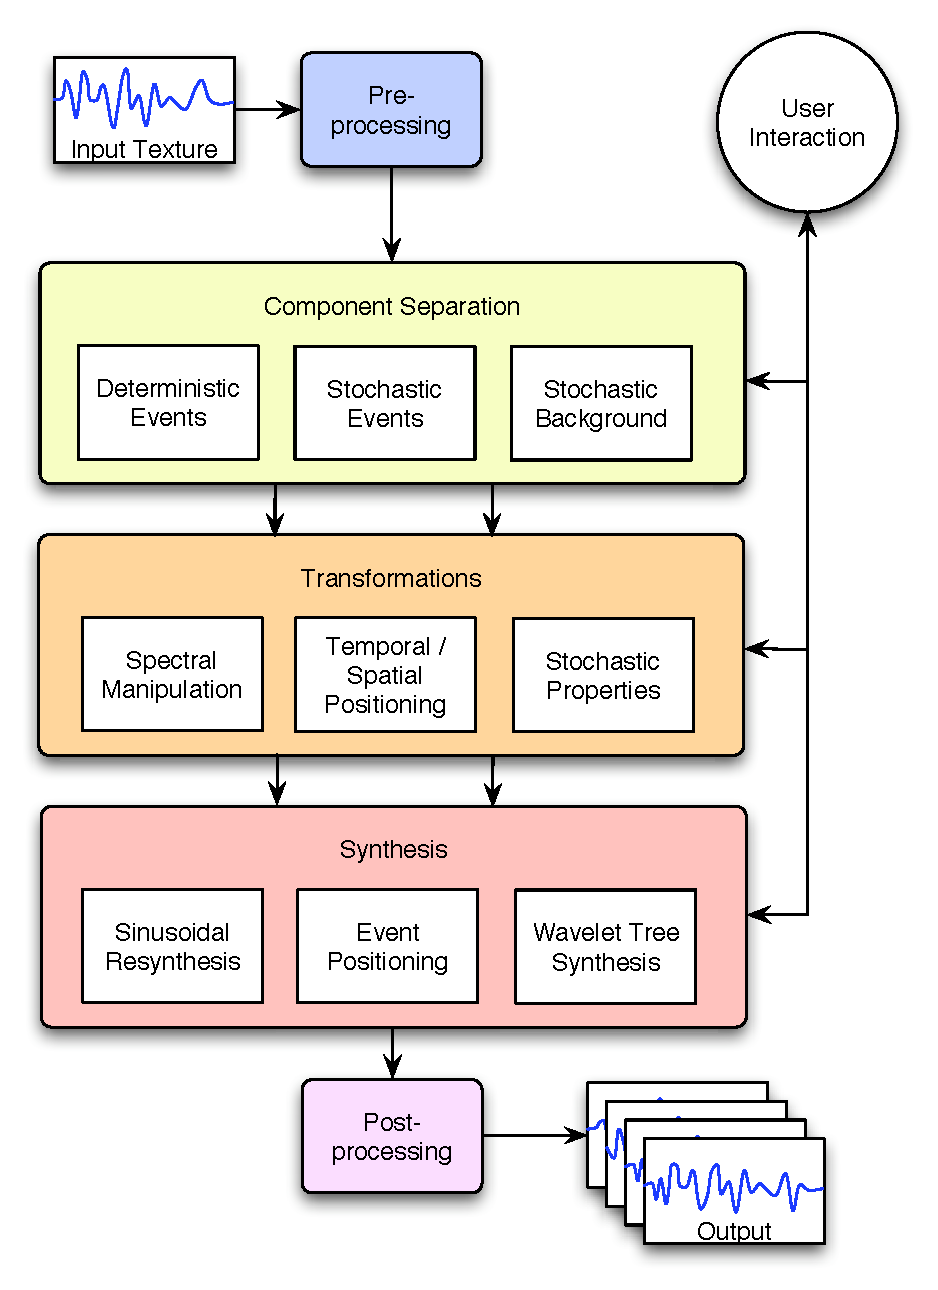
\includegraphics[width=.95\columnwidth]{ourpipeline.eps}
\caption{Stages in our pipeline: The preprocessed sound is analyzed to enable component separation. These components undergo optional transformations before they are individually synthesized and combined to produce the final sound.}
\end{figure}

\subsection{Transformation/Synthesis}
During transformation, the system or user parametrically specify how to 
construct and synthesize the output sound scene.  For foreground
events, transformations include high-fidelity frequency/magnitude-warping, 
time-stretching, and transformations that control the temporal and spatial 
density of event instances.  For background textures, it is possible to parametrically
alter the "similarity" of the sound to the original template.

For example, if we take a single "child yelling" event template from our 
street scene, we make different instances of the event with varying 
loudness, frequencies and durations.  We can then specify for them to occur 
according to some probability, or as a group (child yelling at different 
pitches and times to sound like many children).  Furthermore, we can pan 
each instance differently so that it is perceived as originating from a 
different point in space. The user can experiment with each of these and 
preview the result before the final reconstruction / synthesis stage.  
Transformations on events and background are discussed in Section 5.

%(TODO: need to show scripting language or user interface here or earlier)

The reconstruction / synthesis stage takes event and background templates,
and produces the output texture according to specification.
The stochastic background texture is repeatedly decomposed and 
recomposed (using wavelet tree learning) into new,
perceptually similar, non-repeating stochastic background textures, 
which are layered with the foreground of deterministic events.  From the 
original park sound template, it is possible to generate an arbitrary length 
sound scene with similar background and distribution of events.  Also, the 
loudness, frequency-content, density, and spatialization of each 
component can be controlled and modified independently.  From the same 
template, we can thus generate a new sound scene that gives the impression 
of a park with many more children, or that of a less crowded area with more geese 
than people. We can also vary the parameters dynamically to gradually transform 
from one to the other.

TAPESTREA includes a graphical user interface for performing analysis on 
multiple sounds, and transforming and resynthesizing the components to 
create new sound scenes. Waveform, spectrum and spectrogram displays in 
the analysis view allow users to easily select events to extract. The 
transformation/synthesis view depicts the separated components as 
templates and allows the user to manipulate each template separately or 
group multiple templates together. The interface also provides a means 
for controlling analysis, transformation and synthesis parameters in 
real-time. 

%what a messy pile of words.  YES!!

%The Pipeline

%   3.1 pipeline\\
%       --- input\\
%       --- analysis, event separation\\
%       --- transformation\\
%       --- synthesis\\
%       --- output\\
%       --- control points\\
%   3.2 list of contribution\\


\section{Event Identification and Isolation}

The first step in our framework is to identify and separate the \textit{deterministic events}
from the background noise. In this context, deterministic events are the sinusoidal or pitched 
components of a sound. We separate these since listeners perceive them as distinct 
occurrences against the background of more stochastic, unpitched parts of 
the sound texture. A sound scene may also contain transient, non-sinusoidal events such as footsteps, which are extracted separately by a transient detector. 
%(TODO: write this). 

%\subsection{Preprocessing}

%We are considering several ways of preprocessing the given sound 
%texture to enhance deterministic and transient event extraction. One strategy is to bandpass-filter 
%the sound and perform event detection separately on each subband. This 
%could be useful because what is perceived as an event may differ according 
%to the spectral range in which it takes place. For example, high-frequency
%sounds
%(specific range?)
%are easier to detect than low-frequency sounds of 
%the same magnitude (I think). So processing each subband separately allows 
%for better fine-tuning of the event detection / tracking parameters.
%
%Another form of preprocessing is to intelligently segment the given sound 
%texture using the MARSYAS framework. Each segment could then be processed 
%separately. Since each segment is a contiguous-time clip with uniform 
%features, doing this could also aid event identification.
%
%The thing we actually do is block DC.
%
%\subsection{Classification}
%
%PROBABLY DITCH CLASSIFICATION, AND LEAVE IT FOR FUTURE WORK.
%As described earlier, classification of 
%sounds can give us hints on the appropriate parameters or techniques to use for event detection and 
%tracking. We can classify based on various features, including power, spectral centroid and 
%rollof, spectral flux, zero crossing rate, and Mel-Frequency Cepstral Coefficients. For 
%domain-specific tasks, features such as Parametric Pitch Histogram, and Beat/Periodicity 
%Histogram can be calculated and used. These features also aid segmentation of the original 
%sound, as described in Section 4.1.

\subsection{Sinusoidal Modeling}

To identify deterministic events, we perform sinusoidal analysis based on the spectral 
modeling framework. The sound texture is divided into possibly overlapping 
frames, each of which is transformed into the frequency domain using the 
FFT and processed separately by the sinusoidal analysis framework.

%The lowest frequencies in the spectral frame are eliminated to avoid 
%artifacts from the transform and windowing.
The maximum and average 
magnitudes of the spectral frame are computed and stored. The following 
steps are then repeated until either a specified maximum number of peaks 
have been located or no more peaks are present:
%(kind of ambiguous)(why?)

(1) The maximum-magnitude bin in the frame is located.\\
(2) If the ratio of its magnitude to the average magnitude of the frame is 
below a specified number, it is assumed to be noise and we deduce that no 
more peaks are present.\\
(3) If its magnitude is above a specified absolute threshold, it is added as a sinusoidal peak and the bins it covered are zeroed out in the analysis frame.

Once all the peaks in all the frames have been detected, we match peaks 
from frame to frame if they occur at sufficiently similar frequencies. 
Over time this yields tracks of peaks lasting across frames. The 
matching and updating of tracks takes place in the following way:

(1) Each existing track from previous frames selects a current peak that is 
closest to it in frequency. If the difference in 
frequency is above a reasonable error amount, that track is considered dormant 
and the selected peak remains unmatched.\\
(2) All remaining current peaks that have not been matched to a track are 
added as new tracks, and all existing tracks that have not found a 
continuation are removed if they have remained dormant for several frames.\\
(3) Tracks that continue across several frames are accepted as 
deterministic events.

\begin{figure}[h]
\centering
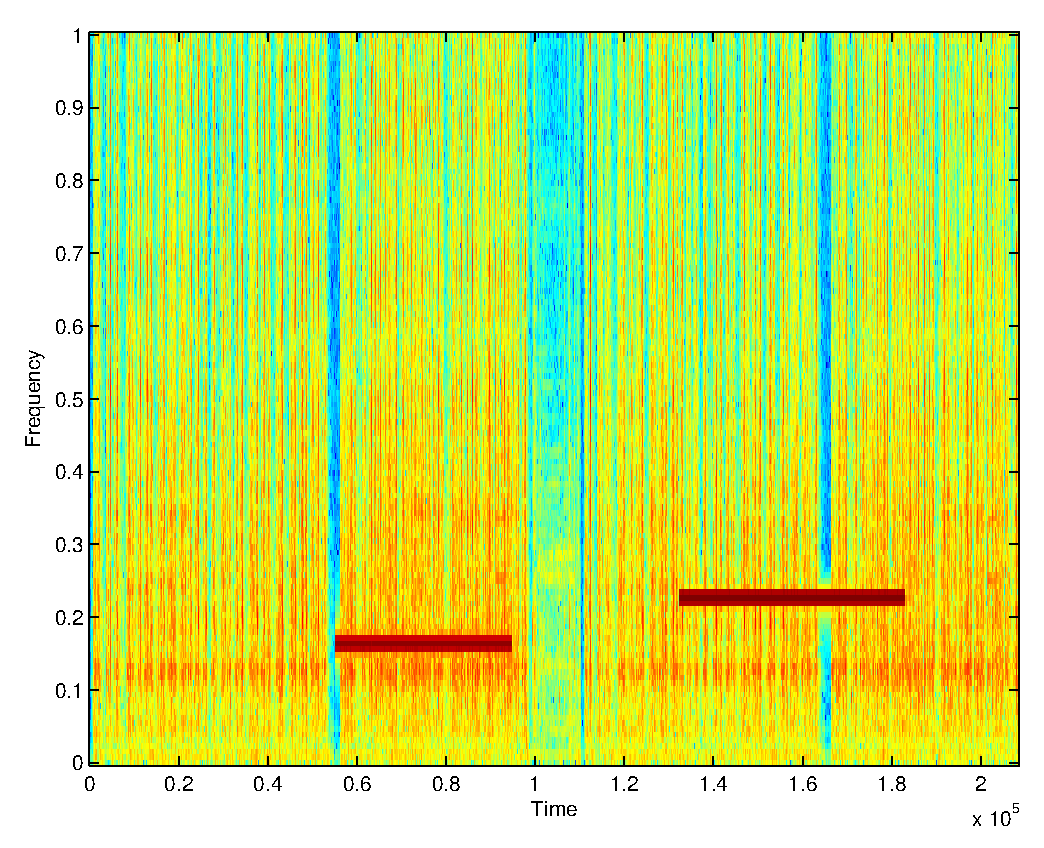
\includegraphics[width=.95\columnwidth]{story1.eps}
\caption{Sinusoids - didactic sms figure waterfall.eps}
\end{figure}

\subsection{Transient Detection}

Transients are brief stochastic sounds with high energy. In a 
spectrogram, a transient occurs as a vertical line, representing the 
simultaneous presence of information at many frequencies. We use a 
transient detector that processes an envelope of a given sound to locate 
points where transients occur.

\subsection{Event Representation}

Deterministic events are represented as sinusoidal tracks. For each 
event, we have access to a history of its frequency, phase and magnitude 
over frames, as well as the times of its onset and completion. 
%An extension based on this information would 
%be to identify sinusoidal tracks that move in similar ways across the same 
%frames, and group them as a single event or object.

Transient events are segmented and isolated sound events from the input sound.
Since they are, by definition, not captured by deterministic event isolation, they cannot be
represented as sinusoidal tracks. Instead, they are stored as sound files that can be read and processed by the system. 
%Once a transient event is detected in the background
%texture, it is isolated in both time and frequency range, and stored as frames of time-varying
%Fourier spectra.  This representation is not as flexible as sinusoidal tracks but represents
%transients better, since they tend to be more noisy than deterministic events, and is amenable
%to spectral transformations.

\subsection{Residual Extraction}

The residue, or non-sinusoidal component, is extracted after the sinusoidal events have been identified. The nearest 
local minima before and after a sinusoidal peak represent the peak's beginning and end respectively. We eliminate 
each peak in a sinusoidal track from the corresponding frame's spectrum by doing linear interpolation on the 
magnitude of the bins between the beginning and end of the peak. We also randomize the phase in these bins.

\section{Transformations}

Heading in the Transformation stage, we now have: (1) deterministic event 
templates, isolated in time and frequency from the 
background, (2) stochastic background sound texture, and (3) transient events.

During transformation, the system or user parametrically specifies how to 
construct and synthesize the output sound scene(s).  The deterministic 
events, transient events and background are modeled and transformed 
separately. The power of the parametric model comes from the 
fact that each transformation is applied independently of others, and each component is 
modified independent of other components. 

\subsection{Event Transformations}

Since deterministic events are modeled parametrically, we leverage 
a number of powerful SMS techniques for transformation. Our system 
facilitates high-fidelity time-stretching and frequency-warping of 
deterministic events, and magnitude-warping of both deterministic and 
transient events. Since individual events are represented separately, we 
use probability/statistics to model the frequency of their occurrence as 
well as the overall density of many instances of the same event. 
Furthermore, it is possible to pan event instances, giving an impression 
of their respective spatial locations by positioning them appropriately 
on stereo channels. The above transformations apply to both 
deterministic and transient events, and the magnitude-warping and 
spatializing can be applied on the background component as well. 

\subsubsection{Sound Manipulation}

\textbf{Frequency/magnitude-warping} - By stretching or compressing the spectral
data, we can respectively raise or lower the frequency content, without 
affecting the duration of the sound.  For deterministic events with sinusoidal tracks, 
we warp the frequency at each point in the track, with high fidelity for almost any factor 
(limited by our range of hearing).  
%For transient events, for which there is (more or 
%less) only the raw spectral data, the spectrum of each will need to be 
%shifted and interpolated (cite phase vocoder), and stretching by factor > 
%2.0 may produce artifacts.  
For any event instance, the magnitude (loudness) can be scaled uniformly.
%or according to frequency.

\textbf{Time-stretching} - Track-based representations allow us to 
robustly change the duration of a track by almost any factor without 
producing artifacts. Hence, the system increases or decreases the 
duration of deterministic events as requested by modifying the time-to-frequency trajectory of their tracks.
%For events with sinusoidal tracks, we can modify the 
%track's time-to-frequeny trajectory to increase or decrease the duration 
%independent of the frequency.  For track-based representation, it is 
%robust to change the duration by almost any factor without producing 
%artifacts.  For example, (imagine that you) see figure below.  For 
%transient events, a new frame-based trajectory can be computed, which 
%will be overlap/added to produce time-stretching. 

%Statistics???

\subsubsection{Sound Placement}

\textbf{Temporal placement} -  TAPESTREA allows placement of an individual event in time, either explicitly or using 
a probability distribution for repeating events.  
%Explicitly, it is possible to 
%script 
%the occurrences of a particular event and apply other
%transformations independently on each event instance. 
Explicitly, a particular instance of an event can be placed on a timeline by specifying its onset time. The timeline 
may also include other event instances as well as background sound. Transformations can be applied on individual 
objects both before and after placement in time. 
%An alternative is to specify a probability distribution, 
%such as Poisson.
For repeating events, an alternative is to specify a mean event density and a probability distribution 
such as Poisson, selected according to the desired periodicity of the repetition. This allows more automated 
event placement. 

\textbf{Spatial positioning} - While not the focus of this research, it 
is straightforward to spatially position individual events in world 
coordinates.
%Explicitly place (or provide trajectory for) an 
%event instance in space (in world coordinates), and assign a particular 
%spatialization effect by providing something similar to an impulse response
%for the space.  The system can place an event instance any where in world
%space (no occlusions), and calculate for distance attenuation, panning across
%any number of output audio channels, and spatialization if an impulse reponse
%is provided.  NOT THE FOCUS OF THIS RESEARCH.

%\subsubsection{Group Control}

%\textbf{Density} - Specify density, or texture of a group of events; parameters include 
%number of event instances and a probability distribution.  While it's possible to achieve
%this control using temporal placement of individual event instances described previously,
%this offers a more globally-aware control of a sound "crowd".  This lends to easier
%control and more potential for system optimizations for a large number of sound sources,
%such as in Tsingos et. al.  Also, the size of the group can be varied dynamically. 
%(ui or example)

%\textbf{Spatial density} - Specify how to distribute group in space.  
%(need interaction here).

\subsection{Stochastic Background Transformations}

In addition to the magnitude warping and panning described at the 
beginning of this section, the system also provides real-time or 
pre-determined control over the similarity between the background 
obtained from the separation phase and the background generated from 
the corresponding template. In addition, the generated background can play for any 
arbitrary amount of time.
%\textbf{Magnitude-warping and panning} - Similar to transient events' frame-based 
%warping - modify the frequency/magnitude of the background texture (using spectral
%modeling).  This can applied either before or after the stochastic modeling.

%\textbf{Time-stretching} - Slow down or speed up the background characteristics, without 
%changing the pitch.

%\textbf{Similarity to original sound} - Modify how similar the new generated background
%will be to the original background.  A lower index of similarity will allow more randomness
%in the synthesized texture.
% - by modify parameters to wavelet tree\\
%--- threshold / randomness (see below)\\
%- synthesis parameters (LPC for micro-transient)\\

%\textbf{Density}\\
% - some metric of stochastic density.\\

\section{Synthesis}

Once the sound has been separated into events and background, we synthesize a sound scene to fit 
the user's preferences, based on the specified transformations. The background 
component and the events are synthesized separately and combined to produce the 
final texture. By default the synthesized texture emulates the original texture as much 
as possible.

Although we discuss transformation and synthesis in separate sections for clarity, these two 
aspects are very closely related. For example, components can be transformed in certain ways even 
while they are being synthesized. 
%probability model?

\subsection{Stochastic Background Generation}

The background is generated using an extension of the wavelet tree 
learning algorithm by Dubnov et. al. ~\shortcite{Dubnov02}. The sound is 
decomposed into a wavelet tree, where each node represents a wavelet 
coefficient and its depth corresponds to its resolution.  The wavelet 
coefficients are computed using the Daubechies wavelet with 5 vanishing 
moments. A new wavelet tree is then built where each node is picked 
based on the similarity of its ancestors and its first k predecessors 
(nodes at the same depth) to corresponding sequences of nodes in the 
original tree. The learning algorithm also takes into account the amount of 
randomness desired.

We added the option of incorporating randomness into the first step of 
the learning and modified k to be a fraction of the total number of 
nodes at the current depth, instead of a fixed number. We also found 
that we can avoid learning the coefficients at the highest resolutions, 
without perceptually altering the results. Since the wavelet tree is binary, every additional 
level learned approximately doubles the running time. Skipping the highest level learning
layers decreases the running time by close to half. 
%accordingly. 
This optimization allowed us to build a real-time version of the wavelet tree analysis and synthesis. 
In addition, the real-time control over the learning parameters allows 
users to immediately observe the effects of changing specific parameters 
and to adjust them accordingly without restarting the process multiple times.
%SAY HOW MUCH FASTER.

%(TODO: fix this)
%- wavelet tree learning works better because we have already separated out 
%what wavelet tree is not good at handling - harmonic events.

\subsection{Event Synthesis}

The deterministic events are synthesized from their representative tracks with 
sinusoidal resynthesis. We linearly interpolate frequency and magnitude 
between consecutive frames before computing the time-domain sound from 
these. 

Deterministic events can be placed in the synthesized texture according to their 
distribution in the original texture, as shown by Zhu and Wyse 
~\shortcite{Zhu04}. In our system, the user can request more instances of a 
certain type of event or less of another, for a customized sound 
scene. 
%For example, a view of the spectral domain over time shows 
%distinct peaks, or events, that the user can select. 
An event can also be 
synthesized and played in isolation so that the user can listen to it 
before deciding its role in the final scene.

Transient events can be directly mixed in to the output after any 
desired magnitude changes, panning and periodicity or density parameters 
have been specified. 

%example and figure

\subsection{Putting It All Together}

% The background and events are mixed. 
% At this point the user can sit back and enjoy 
% the display, or interactively fine-tune it, 
% depending on the degree of involvement with which 
% he is most at ease.    
%FIX THIS.  SAY THAT WE CAN
%SYNTHESIZE INFINITE BACKGROUND USING THE WAVELETS,
%AND ADD IN PREVIOUSLY EXTRACTED EVENTS.  CRAFT, 
%SCULPT, DRIVE FROM ALGORITHM (GAME OR ANIMATION),
%ETC.

To construct a sound scene from the components, background and events are combined 
according to the user's preference. Both the level of involvement required and the 
length of the synthesized sound are flexible. 

A sound scene of a specified length can be generated by placing components 
on a timeline of the desired length. Moreover, we can generate infinitely long sound 
scenes. The modified wavelet algorithm sythesizes infinite background texture (until it 
is stopped), while previously extracted events can be temporally placed against the 
background either with fine control or in an automated manner as described in Section 5.1.2. 

This framework adapts to many techniques for synthesizing the final sound. A user may 
craft a sound scene by listening to and adjusting the components separately, based on how they 
sound as a group or individually. The combined sound can then be similarly sculpted. On the other 
hand, the synthesis can also be driven from a game or animation algorithm that specifies 
transformations according to external occurrences.

%Minimal involvement entails stating the parameters at a high level and 
%allowing the various components to do their job. More low-level control 
%would involve listening to and adjusting the synthesized components 
%separately, and then doing the same with the combined sound texture. 
%Some hybrid between these two approaches may also be possible.

\section{User Interface}

%Unofficially known as abuser interface.
%figure goes here.  it looks like this:
%... (each dot is a track)
The user interface is separated into two phases: analysis and synthesis. Figure 4 (sadly non-existent) 
shows screen shots of both phases. In the analysis stage, the user can load a sound file and view its waveform, frame-by-frame spectrum and spectrogram. These views allow the user to visually identify events and perform analysis on appropriate time and frequency regions to extract specific events. The waveform is useful for identifying areas of high energy in the time domain, which may constitute events such as sudden loud noises. The frame-by-frame spectrum presents a clear view of the sinusoidal peaks in a given frame, and also demonstrates how peak locations change from frame to frame. Associated with this view is the absolute magnitude threshold control (Section 4.1), which can be visually adjusted and given a spectral tilt according to the characteristics of the observed spectrum. Finally, the spectrogram combines time- and frequency-domain information in one view. This makes it easy to identify both sinusoidal events (horizontal lines) and transient events (vertical lines). Time and frequency bounds for the analysis can be specfied by adjusting range sliders in the waveform and spectrum views or by selecting a rectangle in the spectrogram view. In addition, direct control over various other sinusoidal analysis parameters is also available. These parameters have default values that have worked well for a range of sounds. 

Once the user has adjusted the analysis parameters or chosen to use the default setting, analysis can be started by clicking a button. The extracted events are then played separately, along with a frame-by-frame view of their spectrum. The residue can be similarly played and viewed. When the user is satisfied with an extracted event or background, she can save it as a template for use in the synthesis phase and proceed to perform further analysis on the same source sound or a different one.

The synthesis phase of the interface offers a framework for applying transformations as well as synthesizing the resulting sounds. Templates saved from the analysis stage are available in the synthesis stage for listening, transforming, and placing in a sound scene. Templates can be of the following types:\\
(1) Deterministic events\\
(2) Transient events\\
(3) Stochastic background\\
(4) Loops\\
(5) Timelines

The first three are imported directly from the analysis results and the transformations available for these are detailed in Section 5. Loops and timelines help control the temporal placement of components in a sound scene. Any event can be saved as a loop, with parameters that specify how often it repeats and how periodic versus random the repetition is. Individual event instances within a loop can also be randomly transformed within a controllable range, so that every iteration of the loop sounds slightly different. This is useful in generating "`crowd"' sounds, such as a flock of birds constructed from a single extracted chirp, or many people from a single voice. 

While loops parametrically repeat a single event, timelines control the temporal placement of any number of components. The duration of a timeline is specified on creation. Subsequently, any existing template can be dragged on to the timeline; its location on the timeline determines when it is synthesized. When the timeline is played, each template on it is synthesized at the appropriate time step and continues for the duration of the timeline. It is also possible to place timelines within timelines, thus capturing details of a sound scene at different temporal resolutions. Any synthesized sound scene can be written to file while it plays, or play forever (until the computer explodes due to operating system flaws).  

\section{Results}

FIX THIS FOR A BETTER FIGURE, BIRDS, KIDS, WHATEVER SHOWS UP BEST IN A 
SPECTROGRAM.  
Figure 1 describes the effect of sinusoidal 
separation. Figure 1(a) shows the spectogram of a sound texture made up 
of two tones (the red horizontal lines) played separately against the 
background of a typewriter sound. After sinusoidal analysis and 
resynthesis, the tones are isolated, as shown in the spectogram in 
Figure 1(b). 

Since the typewriter noise 
(Figure 1(c)) is stochastic, it becomes the background, although the 
individual typewriter clicks could also be interpreted and generated as 
stochastic events. Figure 1(d) is our visualization of a synthesized 
texture based on the sinusoidal separation. The synthesized typewriter 
background is similar but not identical to the original background in 
Figure 1(c). The sinusoidal events are made to occur at different time 
intervals, and last for different amounts of time. Some of them are also 
pitch-shifted.

more figures and results go here.  use imagination.

%\subsection{Implementation}
%       - architecture
\subsection{Sound Examples}
%       - classes of sound\\
Objectively describe example sounds and results. Have some figures. 

%       - put earlier: waveform at various stages of the pipeline\\
%       - (need a web page)\\
\subsection{Evaluation}
%We have not yet evaluated our method since we are still completing the 
%implementation. Primary results are promising. When we get to the 
%evaluation stage, we can judge our system based on either the "actual" 
%similarity of the synthesized texture to the original, or by their 
%perceptual similarity. The former would require identifying or defining a 
%suitable error metric, while the latter would involve designing and 
%conducting (and participating in) a user study. Since our goal is to 
%generate the sound texture that the user wants to hear, a user study is 
%important.  However, a good error metric would also be useful.
%Evaluate above examples.
%Shirley's idea of having someone construct a new sound texture from existing
%ones and an example to replicate. 
%(THe souhd of slence)

%However, a good error metric would also be useful for 
%judging the psychology soundness of the users.

%However, a technical error metric would also be useful for 
%preliminary testing or for contradicting the results of the user study if 
%necessary. 

%       - error metrics\\
%       - user study\\


\section{Conclusion and Future Work}

We have described a framework for synthesizing unlimited length, perceptually-convincing 
sound scenes with separate control over individual foreground events and the background.  
Given an input sound, the system can automatically locate and isolate deterministic 
and stochastic events, which can then be transformed and placed into new sound scenes 
as individual occurrences or in groups.  Our framework 
also allows users to interactively highlight points of interest in the sound to isolate as 
events.  The background texture is also isolated and segmented into reusable templates.  The 
separations allows for components to be transformed independently and provides a means to 
combine specific elements from completely different sound scenes.

Unlike existing approaches, our framework separates a given sound into well-defined 
deterministic, transient, and stochastic components, which fundamentally allows a greater 
level of control over the variety and quality of the synthesized texture.
We also demonstrated an interactive paradigm for building new sounds textures, which include 
iterative refinement of events, interact previews of transformations, grouping, and placement 
in time and space.  Due to the separation, our system is effective in analyzing and 
synthesizing many classes of sounds. %(this is not true at the moment).

While our system has no fundamental restriction on the type of input sound to analyze,
%model,
there are some limitations. When two events have overlapping spectra, it can be hard for the
analysis to distinguish between them. Also, when events have strong deterministic as well as stochastic components, these components get separated and may be difficult to regroup. 
%Can regroup with a timeline, but what if you want them in a loop? Can timelines be in loops?
Of course, the separation can also be viewed as an advantage as it allows components to be mixed in different ways. 
%What about events that have strong deterministic and stochastic 
%components?  What about long time-scale events with complex temporal and spectral behavior?
%Example: like a motorcycle? Also, foreground vocals (such as children singing/yelling) or many 
%musical sounds are difficult to capture faithfully.

Future work includes overcoming these limitations by using more sophisticated event tracking and perhaps providing a more structured framework for grouping components into events. In addition, we would like to combine machine learning techniques to (1) classify events, and (2) allow the system to learn from the user so that it performs better without human assistance over time. Although the current defaults work well in general, machine learning could be used, for instance, to set default parameters based on the characteristics of the sound being analyzed, for even better automated results. 
%(TODO: future work)  COMBINE MACHINE LEARNING TECHNIQUES TO 1) CLASSIFY EVENTS, 2) LEARN FROM THE USER TO DO %BETTER WITHOUT HUMAN ASSIST OVER TIME. (ALTHOUGH IT WORKS PRETTY GOOD WITH THE DEFAULTS, BLAH BLAH).

\bibliographystyle{acmsiggraph}
\nocite{*}
\bibliography{template}
\end{document}

